%Dokumentenklasse "scrbook" - Erweitert um den Verweis auf die Verzeichnisse und Texteigenschaften
\documentclass[chapterprefix=true, 12pt, a4paper, oneside, parskip=half, listof=totoc, bibliography=totoc, numbers=noendperiod]{scrbook}

%Definierung eigener Farben bei nutzung eines selbst vergebene Namens
\usepackage[table,xcdraw]{xcolor}

% Ränder (Standard bottom ca. 52mm anbzüglich von ca. 4mm für die nach oben rechts gewanderte Seitenzahl)
%Anpassung der Seitenränder
%\usepackage[bottom=48mm,left=30mm,right=30mm]{geometry}
\usepackage[bottom=30mm,left=40mm,right=40mm]{geometry}

% Ränder bei Bedarf zeigen
%\usepackage{showframe}

%Tweaks für scrbook
\usepackage{scrhack}

%Blindtext
\usepackage{blindtext}

%Erlaubt die Darstellung von Sourcecode mit Highlighting
\usepackage{listings}

%Erlaubt unteranderem Umbrücke captions
\usepackage{caption}

%Stichwortverzeichnis
\usepackage{imakeidx}

%Kompakte Listen
\usepackage{paralist}

%Zitate besser formatieren und darstellen
\usepackage{epigraph}

%Glossar, Stichworverzeichnis
\usepackage[toc, acronym]{glossaries} % Akronyme werden als eigene Liste aufgeführt

%PDF einfügen
\usepackage{pdfpages}

%Anpassung von Kopf- und Fußzeile
%beinflusst die erste Seite des Kapitels
\usepackage[automark,headsepline]{scrlayer-scrpage}
\automark{chapter}
\ihead{\leftmark}
\chead{}
\ohead{\thepage}
\ifoot*{}
\cfoot[\thepage]{}
\cfoot*{}
\ofoot*{}
\pagestyle{scrheadings}

%Auskommentieren für die Verkleinerung des vertikalen Abstandes eines neuen Kapitels
%\renewcommand*{\chapterheadstartvskip}{\vspace*{.25\baselineskip}}

%Zeilenabstand 1,5
\usepackage[onehalfspacing]{setspace}

%Verbesserte Darstellung der Buchstaben zueinander
\usepackage[stretch=10]{microtype}

%Deutsche Bezeichnungen für angezeigte Namen (z.B. Innhaltsverzeichnis etc.)
%\usepackage[ngerman]{babel}

%Unterstützung von Umlauten und anderen Sonderzeichen (UTF-8)
\usepackage{lmodern}
\usepackage[utf8]{luainputenc}
\usepackage[T1]{fontenc}

%Einfachere Zitate
\usepackage{epigraph}

%Verwendung von Akronymen
\usepackage[printonlyused]{acronym}

%Unterstützung der H positionierung (keine automatische Verschiebung eingefügter Elemente)
\usepackage{float} 

%Erlaubt Umbrüche innerhalb von Tabellen
\usepackage{tabularx}

%Erlaubt Seitenumbrüche mit Tabellen
\usepackage{longtable}

%Vektorgrafiken
\usepackage{tikz}

%Grafiken (wie jpg, png, etc.)
\usepackage{graphicx}

%Grafiken von Text umlaufen lassen
\usepackage{wrapfig}

%Subfigures in graphics
\usepackage{subcaption}

%Ermöglicht Verknüpfungen innerhalb des Dokumentes (e.g. for PDF), Links werden durch "hidelink" nicht explizit hervorgehoben
\usepackage[hidelinks,german]{hyperref}

\usepackage{todonotes}
\newcommand{\todoredefined}[2][]{\todo[color=green, #1]{#2}}

%Used for making definitions and theorems
\usepackage{amsthm}
\newtheorem{definition}{Definition}
\newtheorem{theorem}{Theorem}

%Used for matrices
\usepackage{amsmath}

%Used for blackboard bold
\usepackage{amssymb}

%Einbindung und Verwaltung von Literaturverzeichnissen
\usepackage{csquotes} %wird von biber benötigt
\usepackage[style=alphabetic, backend=biber, bibencoding=ascii]{biblatex}
\addbibresource{references/references.bib}

%-------------------------------Zusätzliche Anpassungen und Modifikationen--------------------------------------------%

%Anpassung der Überschriften
\addtokomafont{disposition}{\rmfamily}

%Zusätzliche Farben
\definecolor{darkgreen}{RGB}{0,100,0}

%Umbenennungen
\renewcommand{\lstlistlistingname}{Quelltextverzeichnis}

%Pluszeichen in der Referenc beim zitieren ausblenden
\renewcommand*{\labelalphaothers}{}

%Anpassugen zur Quelltextdarstellung, kann bei Bedarf überschrieben werden (z.B. wenn unterschiedliche Sprachen zum Einsatz kommen)
\renewcommand{\lstlistingname}{Codeauszug}
\lstset{
	language=Java,
	numbers=left,
	columns=fullflexible,
	aboveskip=5pt,
	belowskip=10pt,
	basicstyle=\small\ttfamily,
	backgroundcolor=\color{black!5},
	commentstyle=\color{darkgreen},
	keywordstyle=\color{blue},
	stringstyle=\color{gray},
	showspaces=false,
	showstringspaces=false,
	showtabs=false,
	xleftmargin=16pt,
	xrightmargin=0pt,
	framesep=5pt,
	framerule=3pt,
	frame=leftline,
	rulecolor=\color{green},
	tabsize=2,
	breaklines=true,
	breakatwhitespace=true,
	prebreak={\mbox{$\hookleftarrow$}}
}

%Anpassungen für das Abkürzungsverzeichnis
\newglossarystyle{dottedlocations}{%
	\glossarystyle{list}%
	\renewcommand*{\glossaryentryfield}[5]{%
		\item[\glsentryitem{##1}\glstarget{##1}{##2}] \emph{##3}%
		\unskip\leaders\hbox to 2.9mm{\hss.}\hfill##5}%
	\renewcommand*{\glsgroupskip}{}%
}

%%Titles - Uncomment one section of titles

%%Used for titleGraduation
\makeatletter

\newcommand*{\logoPathL}[1]{\gdef\@logoPathL{#1}}
\newcommand*{\logoWidthL}[1]{\gdef\@logoWidthL{#1}}
\newcommand*{\logoPathR}[1]{\gdef\@logoPathR{#1}}
\newcommand*{\logoWidthR}[1]{\gdef\@logoWidthR{#1}}
\newcommand*{\gradeType}[1]{\gdef\@gradeType{#1}}
\newcommand*{\firstExaminer}[1]{\gdef\@firstExaminer{#1}}
\newcommand*{\secondExaminer}[1]{\gdef\@secondExaminer{#1}}
\newcommand*{\matrikelnr}[1]{\gdef\@matrikelnr{#1}}
\newcommand*{\submitDate}[1]{\gdef\@submitDate{#1}}

\renewcommand*{\maketitle}{
	\begin{titlepage}
		\newgeometry{left=2.5cm,right=2.5cm,top=3.0cm,bottom=2.5cm}
		\begin{center}
			\begin{figure}[h]
				\begin{minipage}[hbt]{6cm}
					\flushleft
					\ifx\@logoPathL\empty
					\else
					\includegraphics[width=\@logoWidthL\textwidth]{\@logoPathL}
					\fi
				\end{minipage}
				\hfill
				\begin{minipage}[hbt]{6cm}
					\flushright
					\ifx\@logoPathR\empty
					\else
					\includegraphics[width=\@logoWidthR\textwidth]{\@logoPathR}
					\fi
				\end{minipage}
			\end{figure}
			\vfill
			{\Large \@title\par}
			\vskip 0.5cm
			{\large \bfseries Bachelor Thesis\par}
			\vskip 0.5cm
			{\large submitted in fulfillment of the requirements for the degree \\ \bfseries \@gradeType}
			\vskip 0.5cm
			{\large at the}
			\vskip 0.5cm
			{\large University of Bern \\ Institute of Computer Science}
			\vfill
			\begin{flushleft}
				\begin{tabular}[t]{rl}
					Examiner: &\@firstExaminer\\
					\\
					Handed in by: &\@author\\
					\ifx\@matrikelnr\empty
					\else
					Matriculation number: & \@matrikelnr\\
					\fi
					Date of submission: & \@submitDate
				\end{tabular}
			\end{flushleft}
		\end{center}
		\restoregeometry
	\end{titlepage}
}
\makeatother
\logoPathL{} %just leave empty to hide logo
\logoWidthL{0.5}
\logoPathR{resources/uni_bern_logo.jpg} %just leave empty to hide logo
\logoWidthR{1}
\gradeType{Bachelor of Science (B.Sc.)}
\secondExaminer{Max Mustermann}

%%Used for titleResearchPaper
%\makeatletter

\newcommand*{\firstExaminer}[1]{\gdef\@firstExaminer{#1}}
\newcommand*{\subTitle}[1]{\gdef\@subTitle{#1}}
\newcommand*{\researchPart}[1]{\gdef\@researchPart{#1}}
\newcommand*{\matrikelnr}[1]{\gdef\@matrikelnr{#1}}
\newcommand*{\submitDate}[1]{\gdef\@submitDate{#1}}


\renewcommand*{\maketitle}{
	\begin{titlepage}
		\newgeometry{left=2.5cm,right=2.5cm,top=9.0cm,bottom=2.5cm}
		\begin{center}
			\vfill
			{\Large \@title\par}
			{\normalsize \@subTitle\par}
			\vskip 0.5cm
			{\large \bfseries Forschungsprojekt Teil \@researchPart\par}
			\vskip 0.5cm
			{\large an der}
			\vskip 0.5cm
			{\large Hochschule für Technik und Wirtschaft Berlin\\ Fachbereich 4 - Informatik, Kommunikation und Wirtschaft\\ Studiengang Angewandte Informatik}
			\vfill
			\begin{flushleft}
				\begin{tabular}[t]{rl}
					Examiner: &\@firstExaminer\\
					\\
					Handed in by: &\@author\\
					\ifx\@matrikelnr\empty
					\else
					Matriculation number: & \@matrikelnr\\
					\fi
					Date of submission: & \@submitDate
				\end{tabular}
			\end{flushleft}
		\end{center}
		\restoregeometry
	\end{titlepage}
}
\makeatother
%\subTitle{Ein optionaler Untertitel der Arbeit}
%\researchPart{A}

%%Used by all titles
\title{Stable Neo-Hookean Flesh Simulation}
\author{Corina Danja Masanti}
\matrikelnr{15-128-655} % just leave empty to hide number
\submitDate{01.09.2019}
\firstExaminer{Prof. Dr. David Bommes}
%%End Titles

\makeindex[title=Stichwortverzeichnis, options=-s indexstyle.ist, intoc]
\indexsetup{level=\chapter*,toclevel=chapter}

\makeglossaries
\loadglsentries{glossary_and_acronyms.tex}
\setacronymstyle{long-short}

\begin{document}

\pagenumbering{alph} %fix for same identifier warning, character is not show in title
\maketitle

\pagenumbering{Roman}

\chapter*{Vorwort}
Dies ist ein Vorwort \clearpage
\chapter*{Abstract}

\blindtext \clearpage

\tableofcontents \newpage

\pagenumbering{arabic}
\chapter{Introduction}
\section{Motivation}
The goal of this work is for a regular computer science student to give the necessary physical and mathematical background to understand the field of animation.

\section{Structure}
I will start with the background and then go on to the actual paper. \clearpage
\chapter{Background} \label{c:Background}
This chapter will provide the necessary background in continuum mechanics and mathematics in order to understand the next chapters.

In this chapter we will examine the topic of the paper \textit{Stable Neo-Hookean Flesh Simulation}. The goal of the paper was to model deformations for virtual characters that have human-like features.


\section{Notation and Convention}

\subsection{General Notation}
At first we will declare the notation used in this thesis to avoid misunderstandings. We will use the common notation used in continuum mechanics and additionally we will include the declarations in the paper \textit{Stable Neo-Hookean Flesh Simulation}. 
\\
Scalars are represented by regular, normal-weight variables whereas 
tensors and matrices are represented by upper-case bold letters. Vectors will be denoted by bold lower-case variables.


\subsection{Tensor Notation}

Furthermore we will use the tensor notation used in the paper \textit{Stable Neo-Hookean Flesh Simulation}. They decided to to define vectorization vec(.) as column-wise flattening of a matrix into a vector (\cite{Smith:2018:SNF:3191713.3180491}, 12:5) similar to Golub and Van Loan (2012):

\[
\textbf{A} = \begin{bmatrix} a & c \\ b & d \end{bmatrix} \qquad vec(\textbf{A}) = \boldsymbol{\check{a}} = \begin{bmatrix} a \\ b \\ c \\ d \end{bmatrix}.
\]

In order to indicate that we are dealing with a vectorized matrix we will use the symbol $\check{.}$ as shown above.

Additionally we well have to deal with $4^{th}$ order tensors in the following matrix-of-matrices form:

\[
\mathbb{A} = 
\left[\begin{array}{cc}{\begin{bmatrix} a & c \\ b & d \end{bmatrix}} & {\begin{bmatrix} a & c \\ b & d \end{bmatrix}} \\ {\begin{bmatrix} a & c \\ b & d \end{bmatrix}} & {\begin{bmatrix} a & c \\ b & d \end{bmatrix}}\end{array}\right]
=
\left[\begin{array}{cc}{\left[\mathbf{A}_{00}\right]} & {\left[\mathbf{A}_{01}\right]} \\ {\left[\mathbf{A}_{10}\right]} & {\left[\mathbf{A}_{11}\right]}\end{array}\right]
\]

These matrices are denoted by using blackboard bold.

TODO: 2nd order matrix, see paper 4.1 Tensor Notation

\subsection{Summary}
A quick overview of the used notation:

\begin{addmargin}[2cm]{2cm}
a: scalar \\
\textbf{A}: matrix or tensor \\
\textbf{a}: vector \\
vec(\textbf{A}) = $\boldsymbol{\check{a}}$: vectorized matrix \\
\end{addmargin}

\section{Mathematical Background}

Since mathematics plays an important role in our field of interest we will build a solid background in this chapter. A basic understanding of linear algebra is assumed.

\subsection{Matrices}
At first we will discuss the physical or geometrical meaning of some common matrix properties.


\subsection{Singular Value Decomposition}

The singular value decomposition (SVD) will play an important role in the following. It is important for our application since it represents the best possible approximation of a given matrix by a matrix of low rank. This approximation can be looked at as a compression of the data given (\cite{LiesenMehrmann2015}, S. 295).

\section{Continuum Mechanics}
In this section we will give a broad introduction the field of Continuum Mechanics.
In Continuum Mechanics we are less interested in small particles like atoms or molecules of an object but concentrate on pieces of matter which are in comparison very large. We are therefore concerned with the mechanical behavior of solids and fluids on the macroscopic scale (\cite{Spencer1980}, p. 1).


\section{Deformation}
Graphically we can imagine a deformation with the help of a deformation map. In Fig. \ref{fig:deformationmap} we have on the left side an ellipse that signifies an object in its rest state. On the right side in the same image we can see the ellipse in a deformed state. We can map each point from its rest state to the deformed one with the help of the function $\phi$.

\begin{figure}[!htbp]
	\centering
	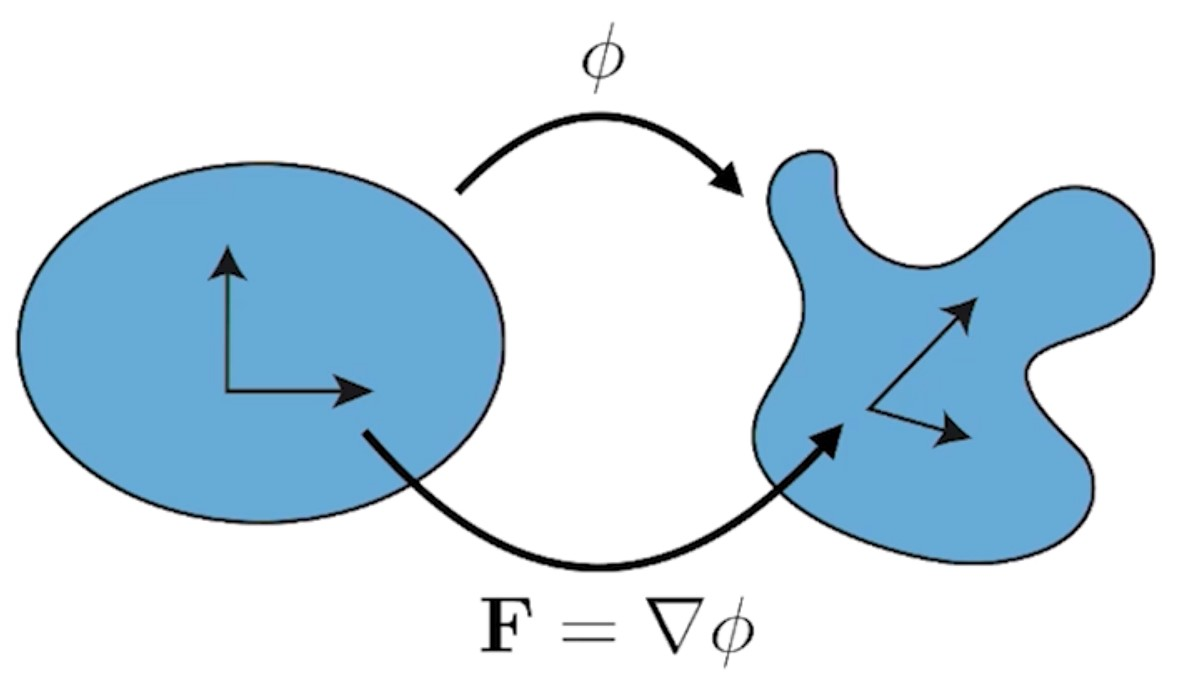
\includegraphics[width=0.5\textwidth]{resources/deformation_map}
	\caption{Deformation Map {\cite{STREAM2018}}}
	\label{fig:deformationmap}
\end{figure}

When applying a force over an object naturally the object itself undergoes a deformation. In the following we will be consistent with most previous literature in continuum mechanics and use the term strain as a measure of deformation and stress as the force per unit area.

\begin{addmargin}[2cm]{2cm}
\textit{Strain = measure of deformation}  \\
\textit{Stress = force per unit area} 
\end{addmargin}


\section{Deformation Gradient}

The deformation gradient $F$ is also shown in Fig. \ref{fig:deformationmap}. It offers us a measurement of the deformation. With its help we can amongst other things calculate the volume and length change an object undergoes during a deformation.
For our needs we define the deformation gradient as followed:

\[
\textbf{F} = \left[ \,f_0\, \bigg| \,f_1\, \bigg| \,f_2\, \right] = \begin{bmatrix} f_0 & f_3 & f_6 \\ f_1 & f_4 & f_7 \\ f_2 & f_5 & f_8 \end{bmatrix}
\]


Measure for the deformation, length and volume change etc.
Nonlinear deformations
http://www.continuummechanics.org/deformationgradient.html
also add some examples

\section{Material Constants}

Naturally the properties of the material the object consists of play an important rule in the deformation process. The two constants $\mu$ and $\lambda$ that are crucial for us are called \textit{Lamé Parameters}. The formula in which they appear is called \textit{Poisso's Ratio} and is of the following form:

\[ \sigma =  \frac{\lambda}{2(\lambda + \mu)} \in [-1, 0.5] \]

The poisson's ratio is of importance for us since it characterizes the materials resistance to volume change. Usually the poisson's ratio of a material is positive.
\\
For the simulation of human-like flesh we have to choose a poisson's ratio that is almost 0.5 to get realistic results.
\\ further reading: http://silver.neep.wisc.edu/~lakes/PoissonIntro.html


\section{Deformation Energy}

In order to get a convincing simulation of high quality we must choose an appropriate energy. In the case of modelling deformations on human-like characters we have to choose an elastic energy. The key property that makes an energy elastic is that if all the forces that are applied over an object add up to zero the object must come back to its rest shape.
\\
The energy then has to be minimized to get the results we want.

\begin{definition}
  This is a definition.
\end{definition}



To include: Piola-Kirchhoff Stress, Cauchy Green invariant, polar decomposition, cauchy green tensor



 \clearpage
\chapter{Background} \label{c:background}

This chapter will provide the necessary background in continuum mechanics and mathematics in order to understand the next chapters.

\section{Notation}
At first we will declare the notation used in this thesis to avoid misunderstandings. We will use the common notation used in continuum mechanics.

\section{Mathematical Background}

Since mathematics plays an important role in our field of interest we will build a solid background in this chapter. A basic understanding of linear algebra is assumed.

\subsection{Matrices}
At first we will discuss the geometrical meaning of some common matrix properties.


\subsection{Singular Value Decomposition}

The singular value decomposition (SVD) will play an important role in the following. It is important for our application since it represents the best possible approximation of a given matrix by a matrix of low rank. This approximation can be looked at as a compression of the data given (\cite{LiesenMehrmann2015}, S. 295).

\section{Continuum Mechanics}
In this section we will give a broad introduction the field of Continuum Mechanics.
In Continuum Mechanics we are less interested in small particles like atoms or molecules of an object but concentrate on pieces of matter which are in comparison very large. We are therefore concerned with the mechanical behavior of solids and fluids on the macroscopic scale (\cite{Spencer1980}, S. 1).

\section{Test}
Nachfolgend der \autoref{lst:helloworld}.

\begin{lstlisting}[caption={Hello World}, captionpos=b, label={lst:helloworld}]
/**
* The HelloWorldApp class implements an application that
* simply prints "Hello World!" to standard output.
*/
class HelloWorldApp {
	public static void main(String[] args) {
		System.out.println("Hello World!"); // Display the string.
	}
}
\end{lstlisting}

\section{Bild}

\begin{wrapfigure}{R}{0.5\textwidth}
	\centering
	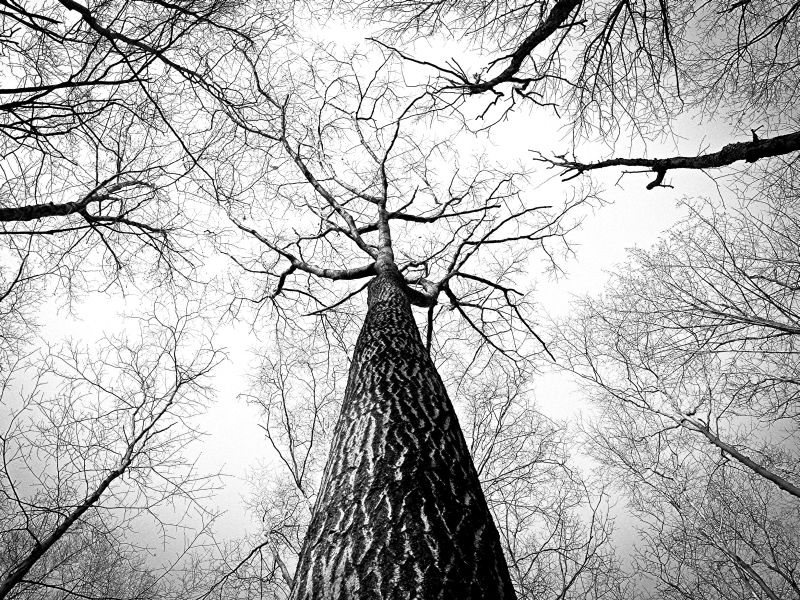
\includegraphics[width=0.5\textwidth]{resources/example}
	\caption{Beispielbild {\cite{PEXELS2015}}}
\end{wrapfigure}

Die rechts zu sehende Grafik demonstriert die Möglichkeiten des Paketes \glqq wrapfig\grqq . Grafiken innerhalb einer \glqq wrapfigure\grqq{} können entweder links oder rechts von Text umlaufen werden.

Die nachfolgende \autoref{img:beispielbild} demonstriert die Darstellung\index{Darstellung} eines \glqq *.jpg\grqq{} Bildes innerhalb des Textes (beim Einfügen kann auf die Endung verzichtet werden, solange der Name einzigartig ist). Zusätzlich enthält dieses einen Untertitel der über das bereits verwendete Label verlinkt werden kann. Der Untertitel\index{Untertitel} erscheint im \gls{abbvz}.

\section{Text Formatierungen und sonstiges}
Dieser Text enthält eine Fußnote\footnote{Fußnoten sind Anmerkungen, die im Druck-Layout aus dem Fließtext ausgelagert werden, um den Text flüssig lesbar zu gestalten.}.

\subsection{Listen}
Listen könne sowohl mit Bullet points als auch mit Zahlen erstellt werden
\begin{itemize}
	\item Eine Liste mit Bullet points
	\item Ein weiteres Element
\end{itemize}

\begin{enumerate}
	\item Eine Liste mit Zahlen
	\item Ein weiteres Element
\end{enumerate}

\subsection{Text Hervorhebungen}
\begin{quote}
	The problem with internet quotes is that you can't always depend on their accuracy \par\raggedleft--- \textup{Abraham Lincoln, 1864}
\end{quote}

"Inspirierende Zitate können mit epigraph eingefügt werden
\epigraph{The problem with internet quotes is that you can't always depend on their accuracy}{Abraham Lincoln, 1864}

Seitenumbrüche können nur direkt nach Text geschrieben werden, sonst lässt sich das Latex nicht mehr compilieren.
\\

\begin{figure}[H]
	\centering
	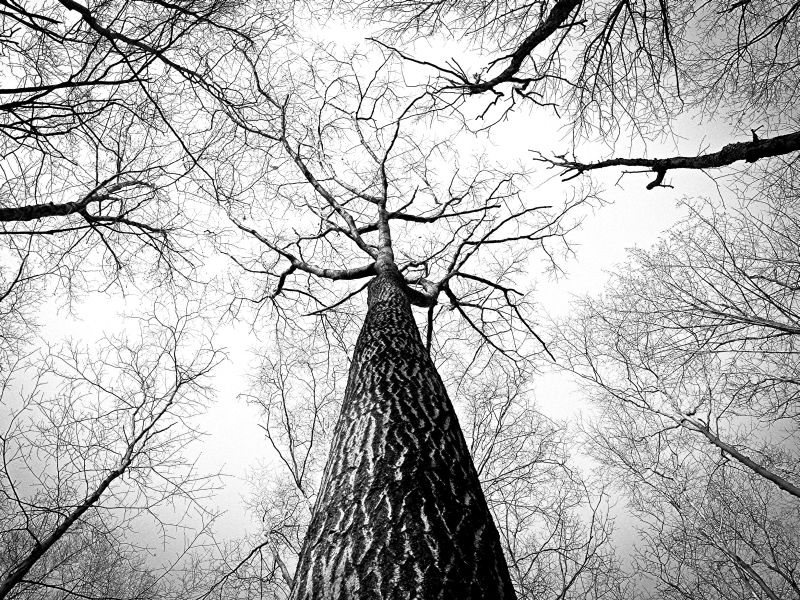
\includegraphics[width=0.7\textwidth]{resources/example}
	\caption{Beispielbild {\cite{PEXELS2015}}}
	\label{img:beispielbild}
\end{figure}

\section{Tabelle}

Nachfolgend \autoref{tbl:DigitalesZertifikat}.

\begin{table}[H]
	\begin{center}
		\renewcommand{\arraystretch}{1.3}
		\begin{tabular}{|l|}
			\hline
			\textbf{Inhaber:}\\
			Alice \\ \hline
			\textbf{Peer (Ersteller):}\\
			Bob \\ \hline
			\textbf{Öffentlicher Schlüssel des Inhabers:}\\
			F2 D2 0E ED FA 4E 9E 0A F2 DD 23 8A 32 44 F3 E9 \\ \hline
			\textbf{Gültigkeit:}\\
			2015-07-01 – 2016-06-30 \\ \hline
		\end{tabular}
	\end{center}
	\caption{Digitales Zertifikat}
	\label{tbl:DigitalesZertifikat}
\end{table}

\section{Long-Table}

Die \glqq Long-Table\grqq kann über definierte Header und Footer über Seitenumbrüche hinweg angezeigt werden.

\begin{longtable}{|l|l|l|l|}
	\hline
	\multicolumn{1}{|c}{\textbf{Version}} & \multicolumn{1}{|c}{\textbf{Codename}} &
	\multicolumn{1}{|c}{\textbf{API}} &
	\multicolumn{1}{|c|}{\textbf{Verteilung}} \\ \hline
	\endfirsthead
	
	\multicolumn{4}{c}{Fortsetzung - Verteilung der Androidversionen (Stand 01.02.2016)}\\ \hline
	\multicolumn{1}{|c}{\textbf{Version}} & \multicolumn{1}{|c}{\textbf{Codename}} &
	\multicolumn{1}{|c}{\textbf{API}} &
	\multicolumn{1}{|c|}{\textbf{Verteilung}} \\ \hline 
	\endhead
	
	\multicolumn{4}{c}{Fortsetzung auf nachfolgender Seite}
	\endfoot
	
	\caption{Verteilung der Androidversionen (Stand: 01.02.2016)}
	\label{tab:androidverteilung}
	\endlastfoot
	
	2.2 & Froyo & 8 & 0.1\%\\ \hline
	2.3.3 - 2.3.7 & Gingerbread & 10 & 2.7\%\\ \hline
	4.0.3 - 4.0.4 & Ice Cream Sandwich & 15 & 2.5\%\\ \hline
	4.1.x & Jelly Bean & 16 & 8.8\%\\ \cline{1-1} \cline{3-4}
	4.2.x &  & 17 & 11.7\%\\ \cline{1-1} \cline{3-4}
	4.3 &  & 18 & 3.4\%\\ \hline
	4.4 & KitKat & 19 & 35.5\%\\ \hline
	5.0 & Lollipop & 21 & 17.0\%\\ \cline{1-1} \cline{3-4}
	5.1 &  & 22 & 17.1\%\\ \hline
	6.0 & Marshmallow & 23 & 1.2\%\\ \hline
\end{longtable}

\section{Literaturverweis}

Weil für die alte\index{alte} und die neue Rechtschreibung verschiedene Trennregeln\index{Trennregeln} gelten, sind Deutsch mit alter Rechtschreibung und Deutsch mit neuer Rechtschreibung zwei verschiedene Sprachen (\cite{Knappen2009}, S. 192).

\section{Onlineverweise}

Siehe Google.de \cite{Google2015}.

\section{Glossar}
Der Glossar enthält die Beschreibung verwendeter Begriffe für das bessere Verständnis gegenüber dem Leser. Beispiele sind: \gls{berlin}, \gls{outsourcing}, \gls{asp}, \gls{policy} und \gls{pcie}.

\section{Abkürzungsverzeichnis}
Das Abkürzungsverzeichnis listet alle verwendeten Abkürzungen auf. Einige Beispiele sind \gls{sas}, \gls{cd}, \gls{lan} und \gls{iso}. Die erneute Verwendung zeigt nur noch die Abkürzung: \gls{sas}, \gls{cd}, \gls{lan} und\index{und} \gls{iso}. \clearpage
\chapter{Paper} \label{c:Paper}
In this chapter we will examine the topic of the paper \textit{Stable Neo-Hookean Flesh Simulation}. The goal of the paper was to model deformations for virtual characters that have human-like features. They concentrated on the deformation energy.

\section{Energy Formulation}

For our needs we need a hyperelastic energy that is stable in the following four important ways:

\begin{itemize}
\item Inversion stability
\item Reflection stability
\item Rest stability
\item Meta-stability under degeneracy
\end{itemize}

\todoredefined[inline]{
TODO: explain each step
}

\subsection{Previous Work}
Here comes previous work in neo-hookean energy formulation. What is neo-hookean and why do we need it here?
And what is wrong with each one.

\subsection{Stable Neo-Hookean Energy}
Conclude to the energy proposed in the paper.

\section{Energy Analysis}
Calculations and Herleitungen

\subsection{First Piola-Kirchhoff Stress (PK1)}
Explain.

\subsection{The Energy Hessian Terms}
Calculations

\subsection{The Tikhonov, Mu, and Gradient Terms}
Calculations

\subsection{The Volume Hessian}
Calculations
 
\subsection{The Complete Eigensystem}
Calculations

\section{Experiments with the Code}
The authors of the paper \textit{Stable Neo-Hookean Flesh Simulation} \cite{Smith:2018:SNF:3191713.3180491} kindly provided the implementation for an application of their formulated energy. In this code they implemented the stretch test on a cube. The output were 26 static images with show the deformation in 25 steps. 

\todoredefined[inline]{
TODO: Explain how the code is implemented in simple words and how the energy is taken in account with the poisson's ratio.
}


The following images show the stretch test with $\mu = 1.0$, $\lambda = 10.0$ and a resolution of 10.0 on a tetrahedral and a hexahedral mesh:

\begin{figure}[!htbp]
	\centering
	\begin{subfigure}[b]{\textwidth}
        \centering
        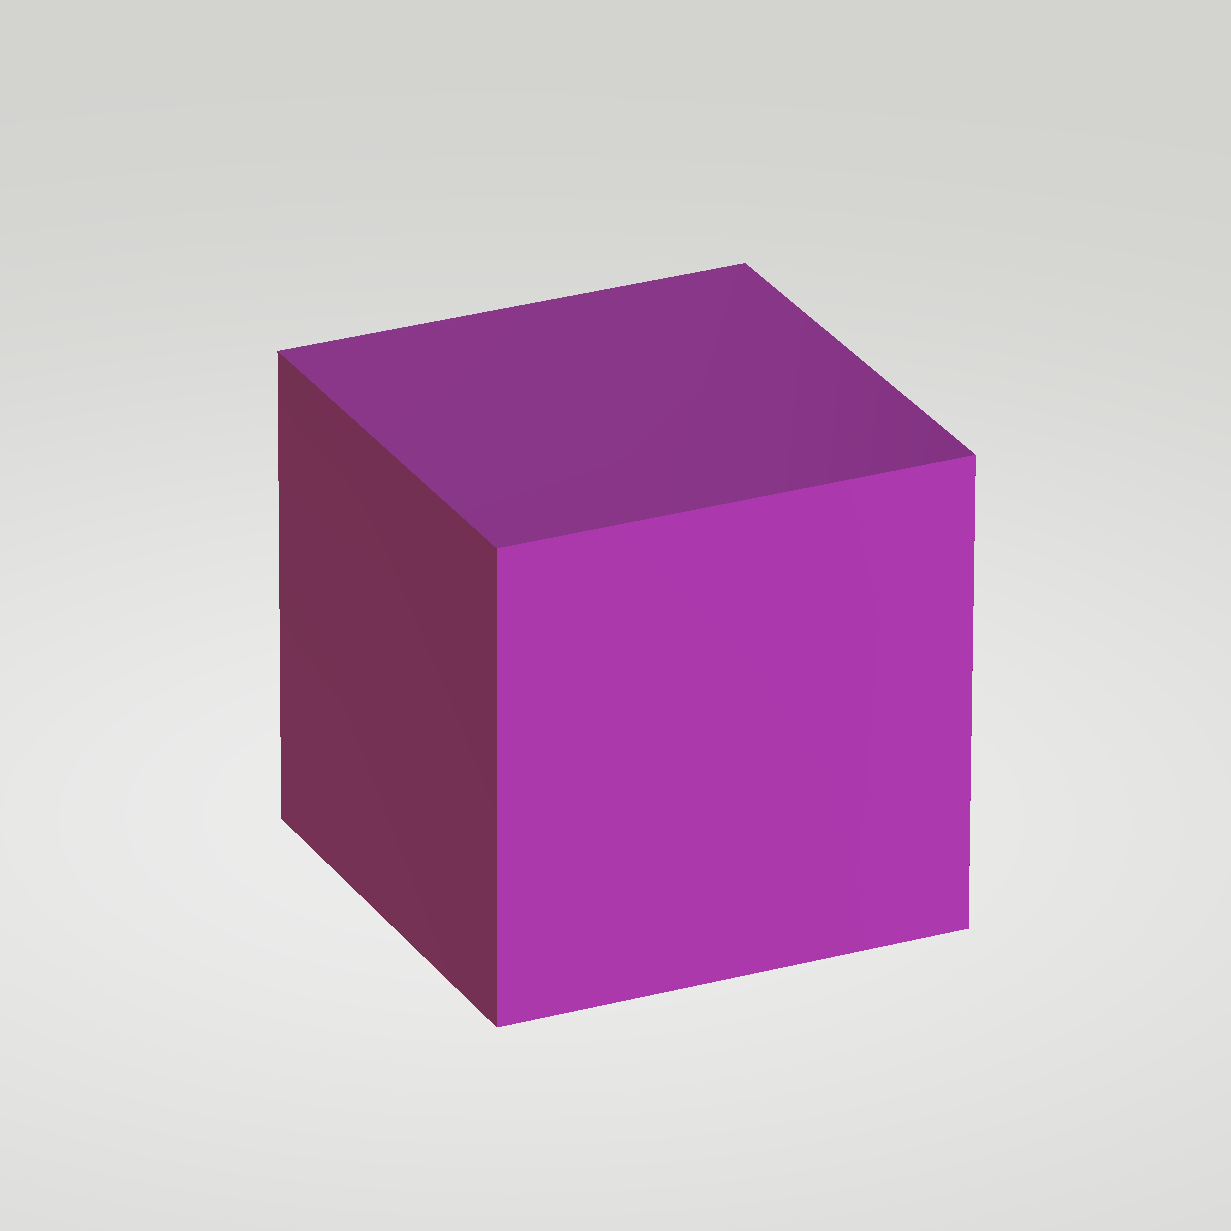
\includegraphics[width=0.24\textwidth]{resources/hexcli_step0.png}
        \hfill
        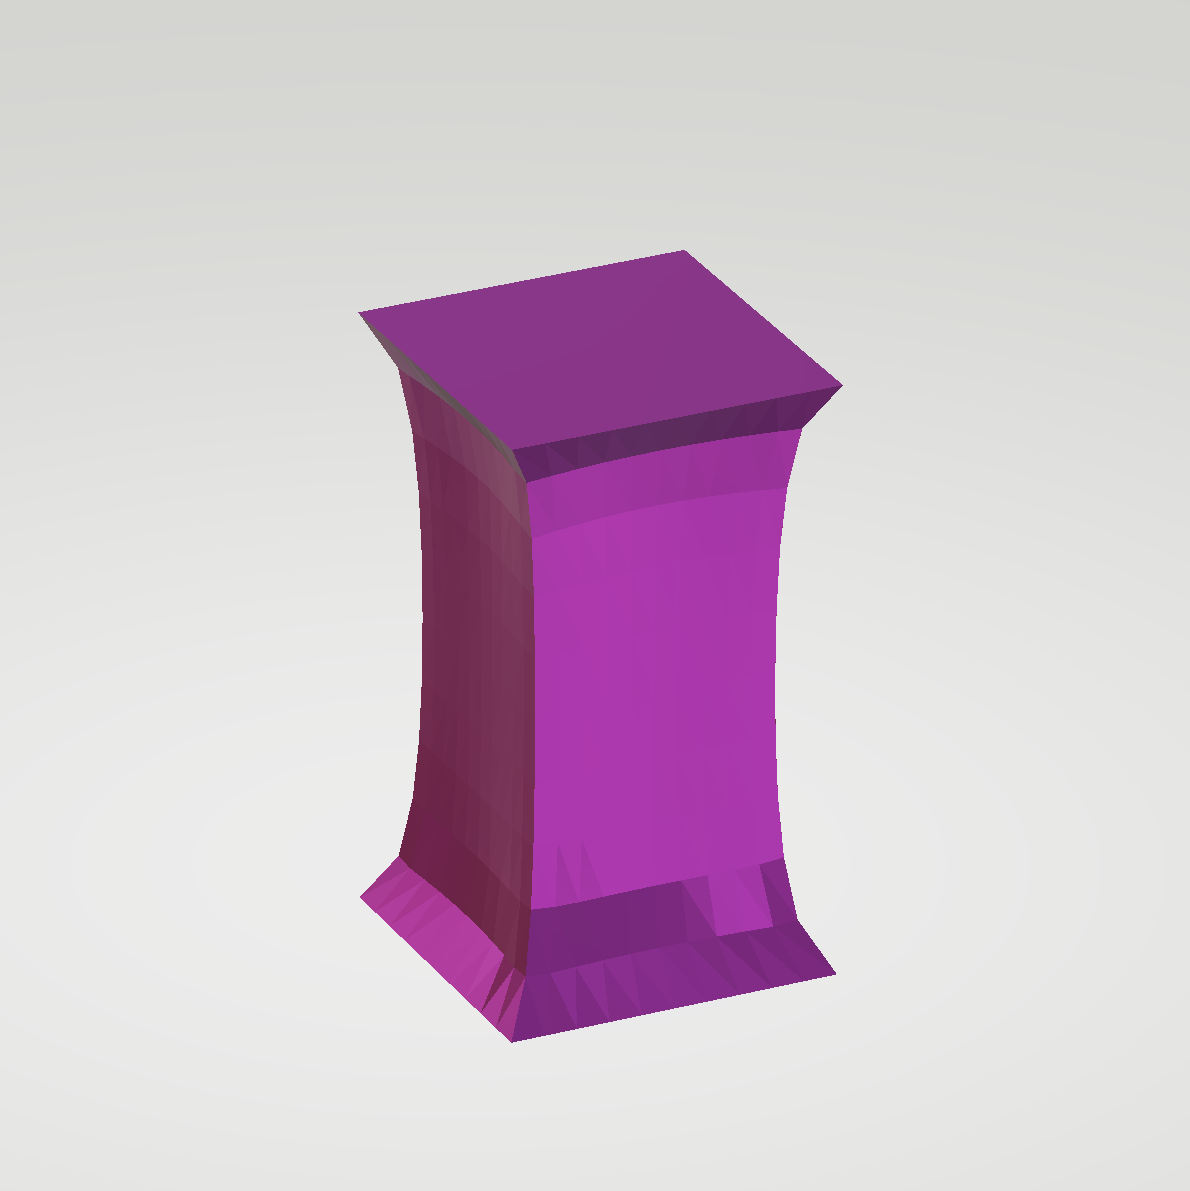
\includegraphics[width=0.24\textwidth]{resources/hexcli_step8.png}
        \hfill
        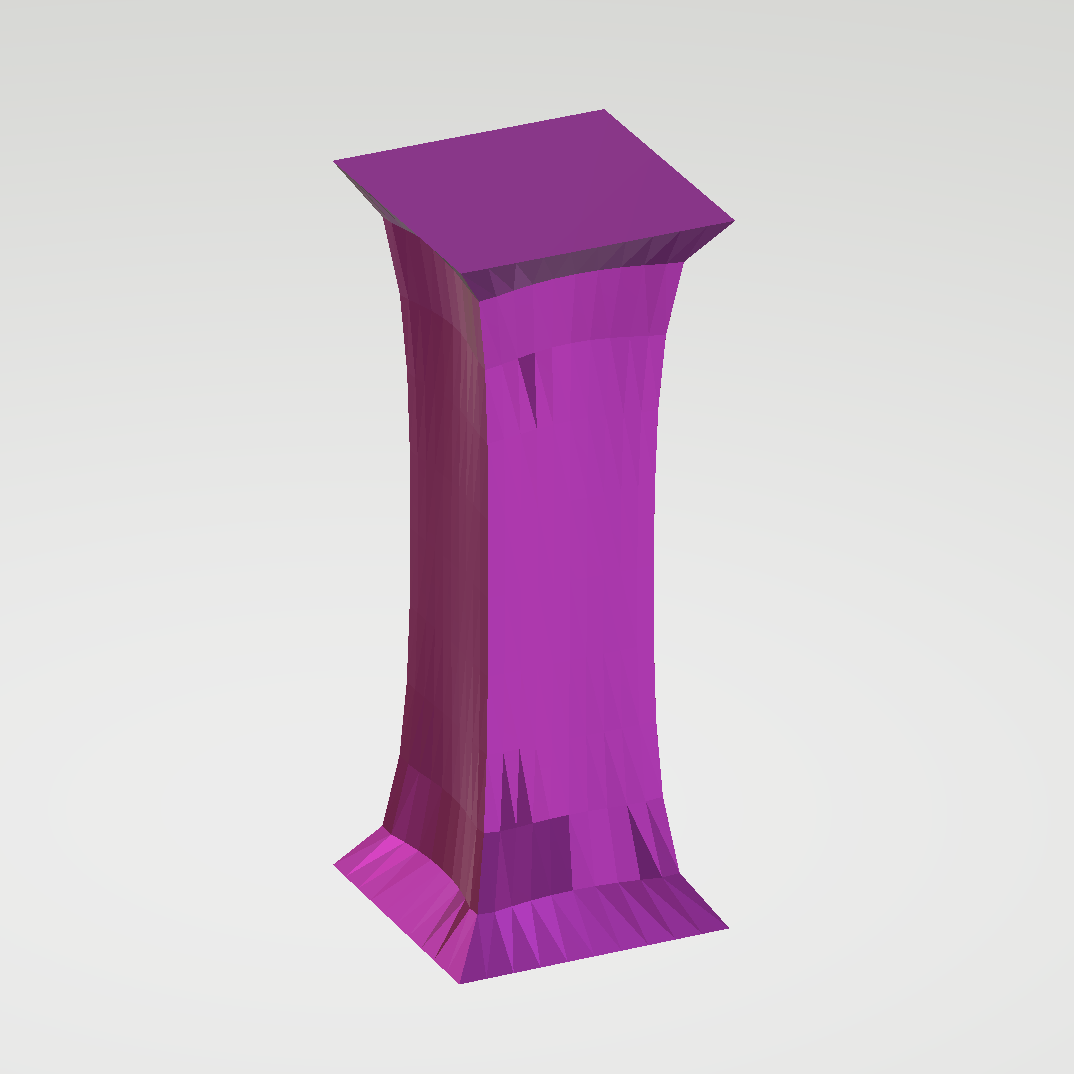
\includegraphics[width=0.24\textwidth]{resources/hexcli_step16.png}
        \hfill
        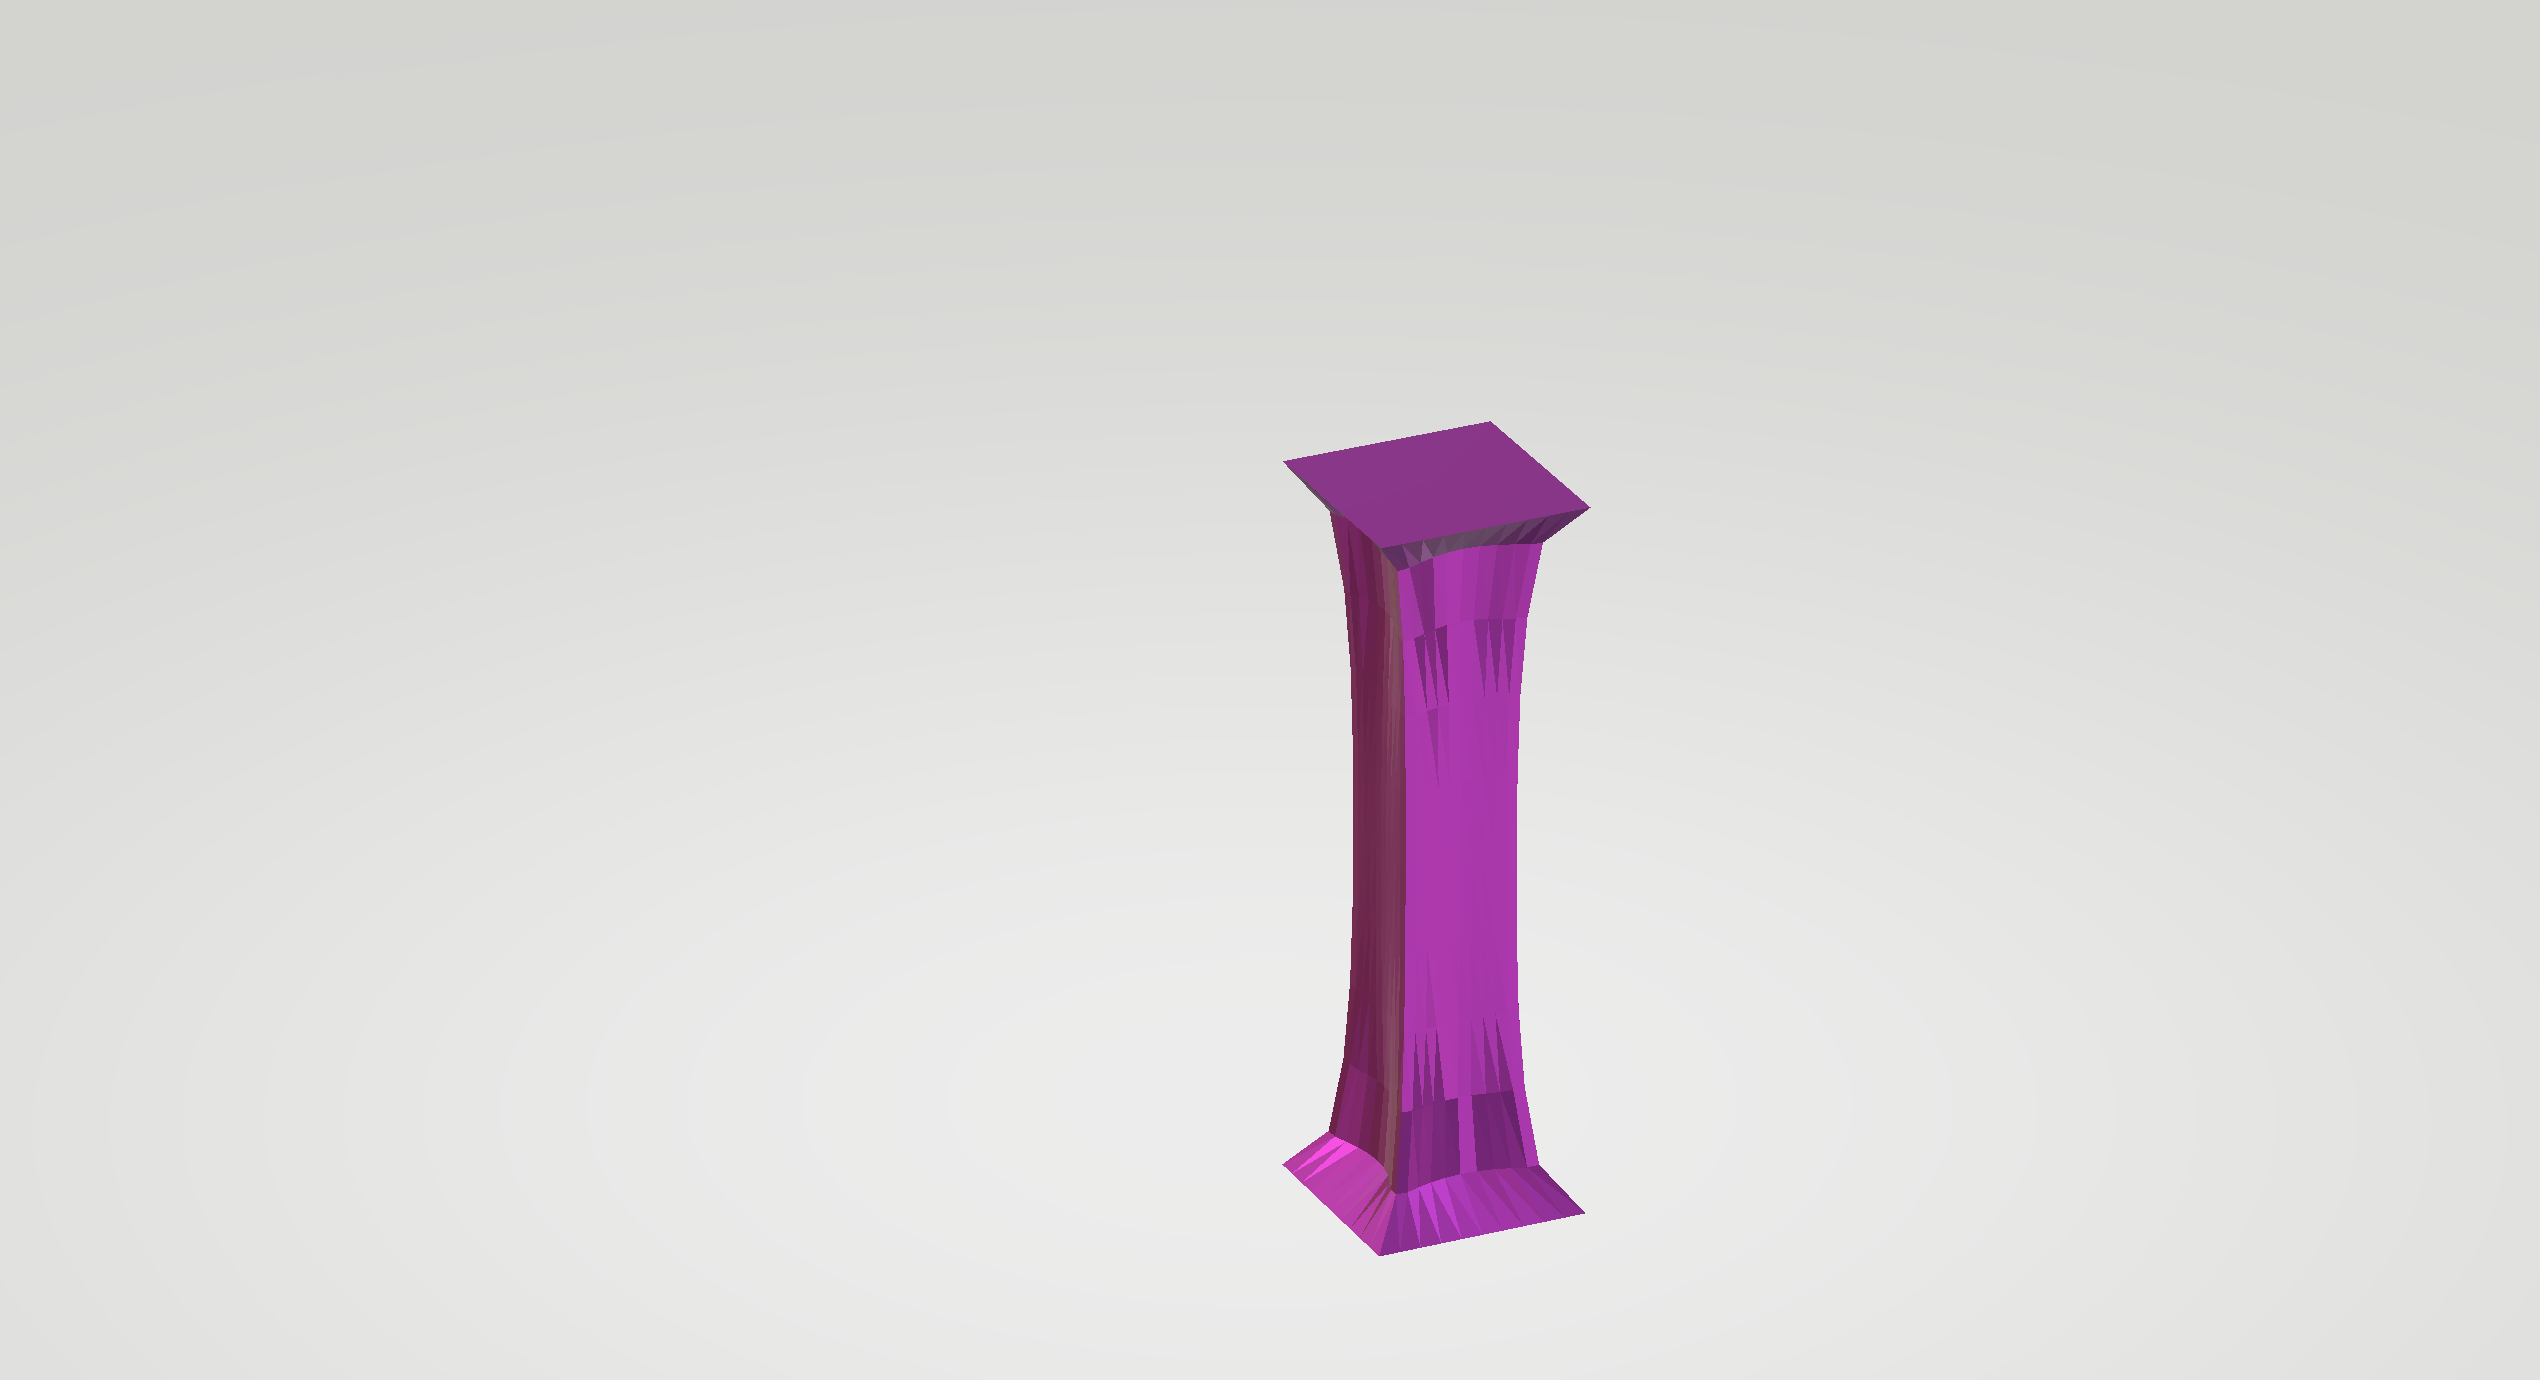
\includegraphics[width=0.24\textwidth]{resources/hexcli_step24.png}
        \caption{Stretch test on a hexahedral mesh}
    \end{subfigure}
    \vskip\baselineskip
    \begin{subfigure}[b]{\textwidth}
        \centering
        
\includegraphics[width=0.24\textwidth]{resources/tetcli_step0.png}
        \hfill
        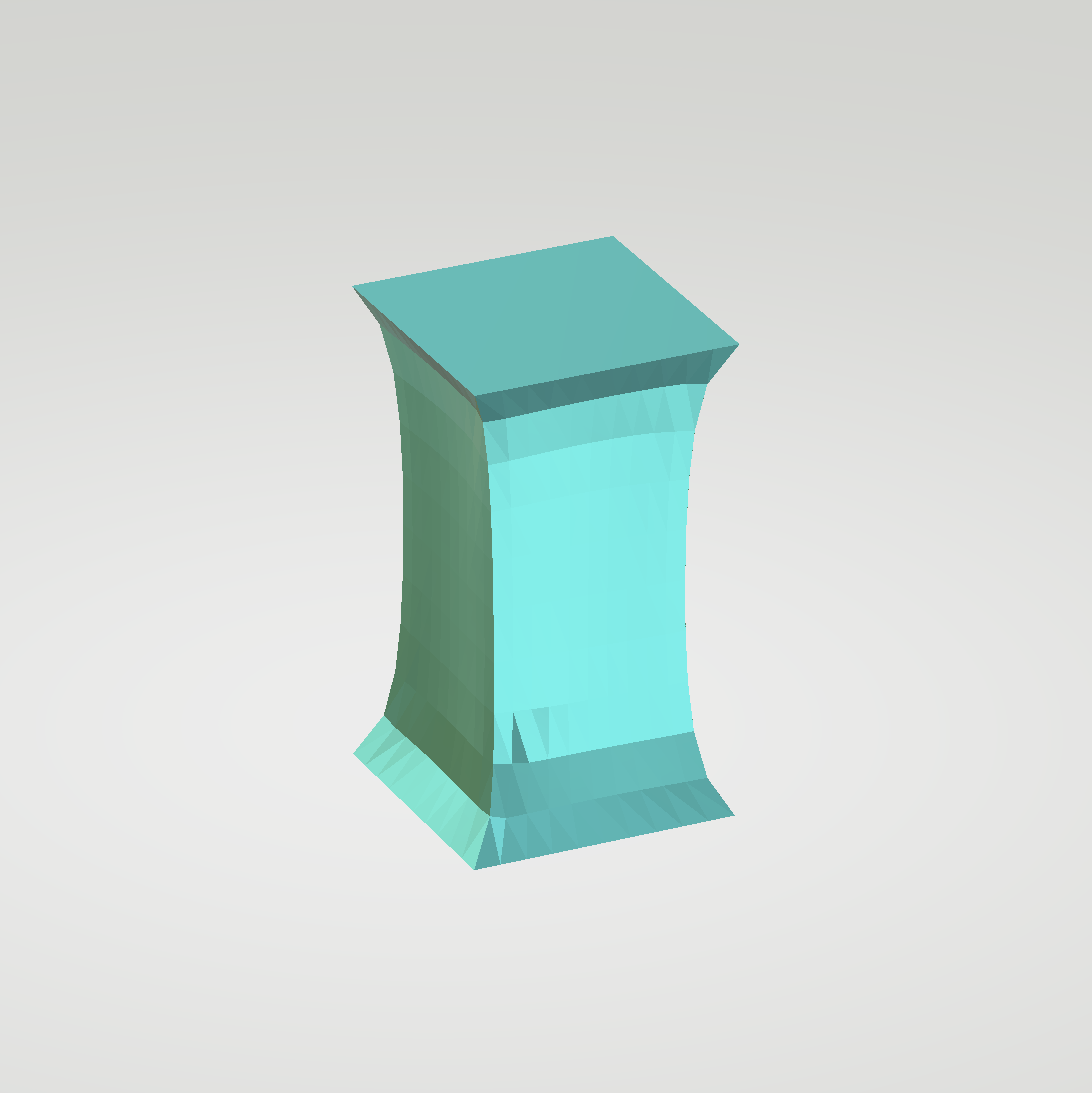
\includegraphics[width=0.24\textwidth]{resources/tetcli_step8.png}
        \hfill
        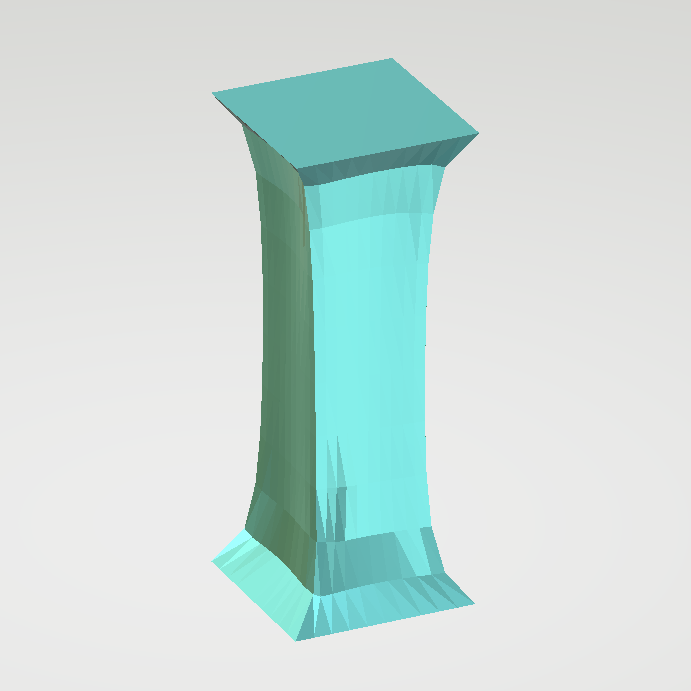
\includegraphics[width=0.24\textwidth]{resources/tetcli_step16.png}
        \hfill
        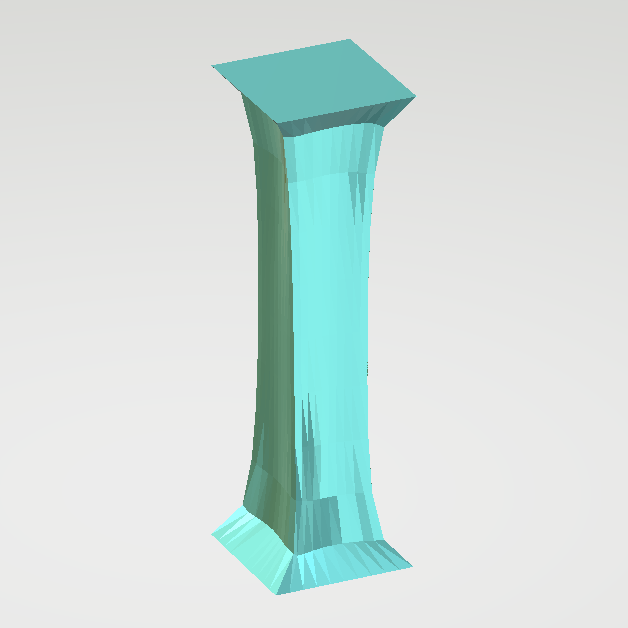
\includegraphics[width=0.24\textwidth]{resources/tetcli_step24.png}
        \caption{Stretch test on a tetrahedral mesh}
    \end{subfigure}
    \caption{Stretch test performed on a cube with (a) a hexahedral mesh and (b) a tetrahedral mesh}
\end{figure}





\section{Discussion}
Stuff, Taylor approx.


 \clearpage

\pagenumbering{Alph}
\listoffigures \clearpage
\listoftables \clearpage
\lstlistoflistings \clearpage

\printindex \clearpage

\printglossary[title={Glossar}] \clearpage
\printglossary[style=dottedlocations,type=\acronymtype,title={Abkürzungsverzeichnis}] \clearpage

\printbibliography[heading=bibintoc, keyword={book}, title={Literaturverzeichnis}]\clearpage
\printbibliography[heading=bibintoc, keyword={online}, title={Onlinequellen}]\clearpage
\printbibliography[heading=bibintoc, keyword={image}, title={Bildquellen}]\clearpage

% Anhang
\appendix

\chapter{}
\addcontentsline{toc}{chapter}{Anhang A}

\section{Diagramm}

\section{Tabelle}

\section{Screenshot}

\section{Graph}

% Eigenständigkeitserklärung
\addchap{Eigenständigkeitserklärung}

Hiermit versichere ich, dass ich die vorliegende Masterarbeit selbstständig und nur unter
Verwendung der angegebenen Quellen und Hilfsmittel verfasst habe. Die Arbeit wurde bisher
in gleicher oder ähnlicher Form keiner anderen Prüfungsbehörde vorgelegt.

\vskip 1cm

Stadt, den xx.xx.xxxx

\vskip 1.5cm

Max Mustermann

\end{document}